\subsection{presenter}
\label{subsec:presenter}

\begin{figure}[H]
  \centering
  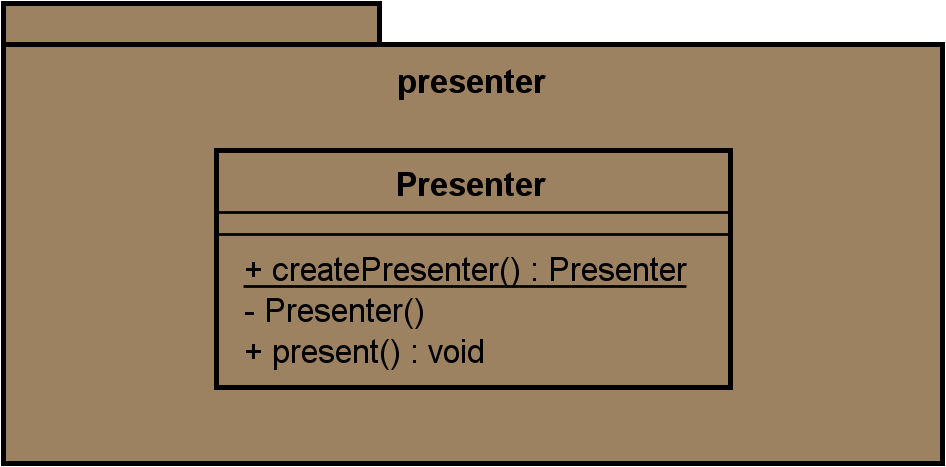
\includegraphics[width=0.6\textwidth]{../diagramimages/presenter.png}
  \caption{presenter-Package}
\end{figure}

\medskip
Der presenter ist für den Aufbau von \gls{programname}, also das
Initialisieren, Instanziieren und Referenzieren aller Programmelemente zuständig.
Er ist sozusagen der ``glue code'' von \gls{programname}.
Er wird im main-Thread von der main-Klasse erzeugt und ruft alle Konstruktoren auf.
In anderen Worten baut er \gls{programname} auf.